\documentclass[a4paper,10pt]{article}
\usepackage[french]{babel}
\usepackage[utf8]{inputenc}
\usepackage[left=2.5cm,top=2cm,right=2.5cm,nohead,nofoot]{geometry}
\usepackage{url}
\usepackage[T1]{fontenc}
\usepackage{float}
\usepackage{afterpage}
\usepackage{amsmath}
\usepackage{graphicx}
\usepackage{tabularx}
\usepackage{csquotes}
\usepackage{fullpage}
\usepackage{pdfpages}
\usepackage{listings}
\usepackage{color}

\usepackage{listings}
\usepackage{mdframed}
\usepackage{color}
\usepackage{pdflscape}
\usepackage{minted}
\usemintedstyle[sql]{native}

\definecolor{mygreen}{rgb}{0,0.6,0}
\definecolor{mygray}{rgb}{0.5,0.5,0.5}
\definecolor{mymauve}{rgb}{0.58,0,0.82}

\lstset{ %
  backgroundcolor=\color{white},   % choose the background color; you must add \usepackage{color} or \usepackage{xcolor}
  basicstyle=\footnotesize,        % the size of the fonts that are used for the code
  breakatwhitespace=false,         % sets if automatic breaks should only happen at whitespace
  breaklines=true,                 % sets automatic line breaking
  captionpos=b,                    % sets the caption-position to bottom
  commentstyle=\color{mygreen},    % comment style
  deletekeywords={...},            % if you want to delete keywords from the given language
  escapeinside={\%*}{*)},          % if you want to add LaTeX within your code
  extendedchars=true,              % lets you use non-ASCII characters; for 8-bits encodings only, does not work with UTF-8
  frame=single,                    % adds a frame around the code
  keepspaces=true,                 % keeps spaces in text, useful for keeping indentation of code (possibly needs columns=flexible)
  keywordstyle=\color{blue},       % keyword style
  language=Octave,                 % the language of the code
  otherkeywords={*,...},           % if you want to add more keywords to the set
  numbers=left,                    % where to put the line-numbers; possible values are (none, left, right)
  numbersep=5pt,                   % how far the line-numbers are from the code
  numberstyle=\tiny\color{mygray}, % the style that is used for the line-numbers
  rulecolor=\color{black},         % if not set, the frame-color may be changed on line-breaks within not-black text (e.g. comments (green here))
  showspaces=false,                % show spaces everywhere adding particular underscores; it overrides 'showstringspaces'
  showstringspaces=false,          % underline spaces within strings only
  showtabs=false,                  % show tabs within strings adding particular underscores
  stepnumber=2,                    % the step between two line-numbers. If it's 1, each line will be numbered
  stringstyle=\color{mymauve},     % string literal style
  tabsize=2,                     % sets default tabsize to 2 spaces
  title=\lstname                   % show the filename of files included with \lstinputlisting; also try caption instead of title
}

\usepackage[pdftex,
            pdfauthor={A. Caccia, A. Madeira Cortes},
            pdftitle={Bases de données - Projet},
            pdfsubject={INFO-H-303 : Bases de données - Projet}]{hyperref}

\linespread{1.1}

\setlength{\parskip}{0.5em}

\begin{document}

\begin{titlepage}
    \begin{center}
        \textbf{\textsc{Université Libre de Bruxelles}}\\
        \textbf{\textsc{Faculté des Sciences}}\\
        \textbf{\textsc{Département d'Informatique}}

        \vfill{}
        \vfill{}

        \begin{center}
            {\Huge INFO-H-303 : Bases de données}
        \end{center}

        {\Huge \par}

        \begin{center}
            {\LARGE Projet : Annuaire d'établissements Horeca}
        \end{center}

        {\Huge \par}

        \begin{center}
            {\large A. Caccia, A. Madeira Cortes}
        \end{center}

        {\Huge \par}
        \vfill{}
        \vfill{}

        {\large\par}
        \vfill{}
        \vfill{}
        % \enlargethispage{3cm} % do not remove

        \textbf{Année académique 2015--2016}
    \end{center}
\end{titlepage}

\section{Introduction}

Le projet consiste en la création d'une plateforme permettant de lister, commenter et noter des établissements horeca. Le but pédagogique étant, bien sur, d'interfacer cette plateforme avec une base de données crée par nos soins, il était important d'utiliser un langage de programmation permettant d'utiliser des requêtes SQL écrites de la même façon que celles vue au cours.

Le langage que nous avons choisi est, in fine, Ruby. Le framework web l’accompagnant est Rails (plus connu sous le nom de Ruby on Rails). 

Nous avons opté de choisir une base de données PostgreSQL, qui est la plus intuitive à utiliser avec Rails (et dont les requêtes conservent le format vu au cours).

Le nom donné à notre application est Welp, déformation du nom ``Yelp''\footnote{\url{www.yelp.com}} qui est un site web fort connu permettant les mêmes fonctionnalités que celles demandées pour ce projet.

MISSING HERE: APPORTS PERSONNELS.

TODO: 

- Mettre à jour traduction relationnelle

- Mettre à jour les contraintes d'intégrité

- Requêtes

\begin{landscape}

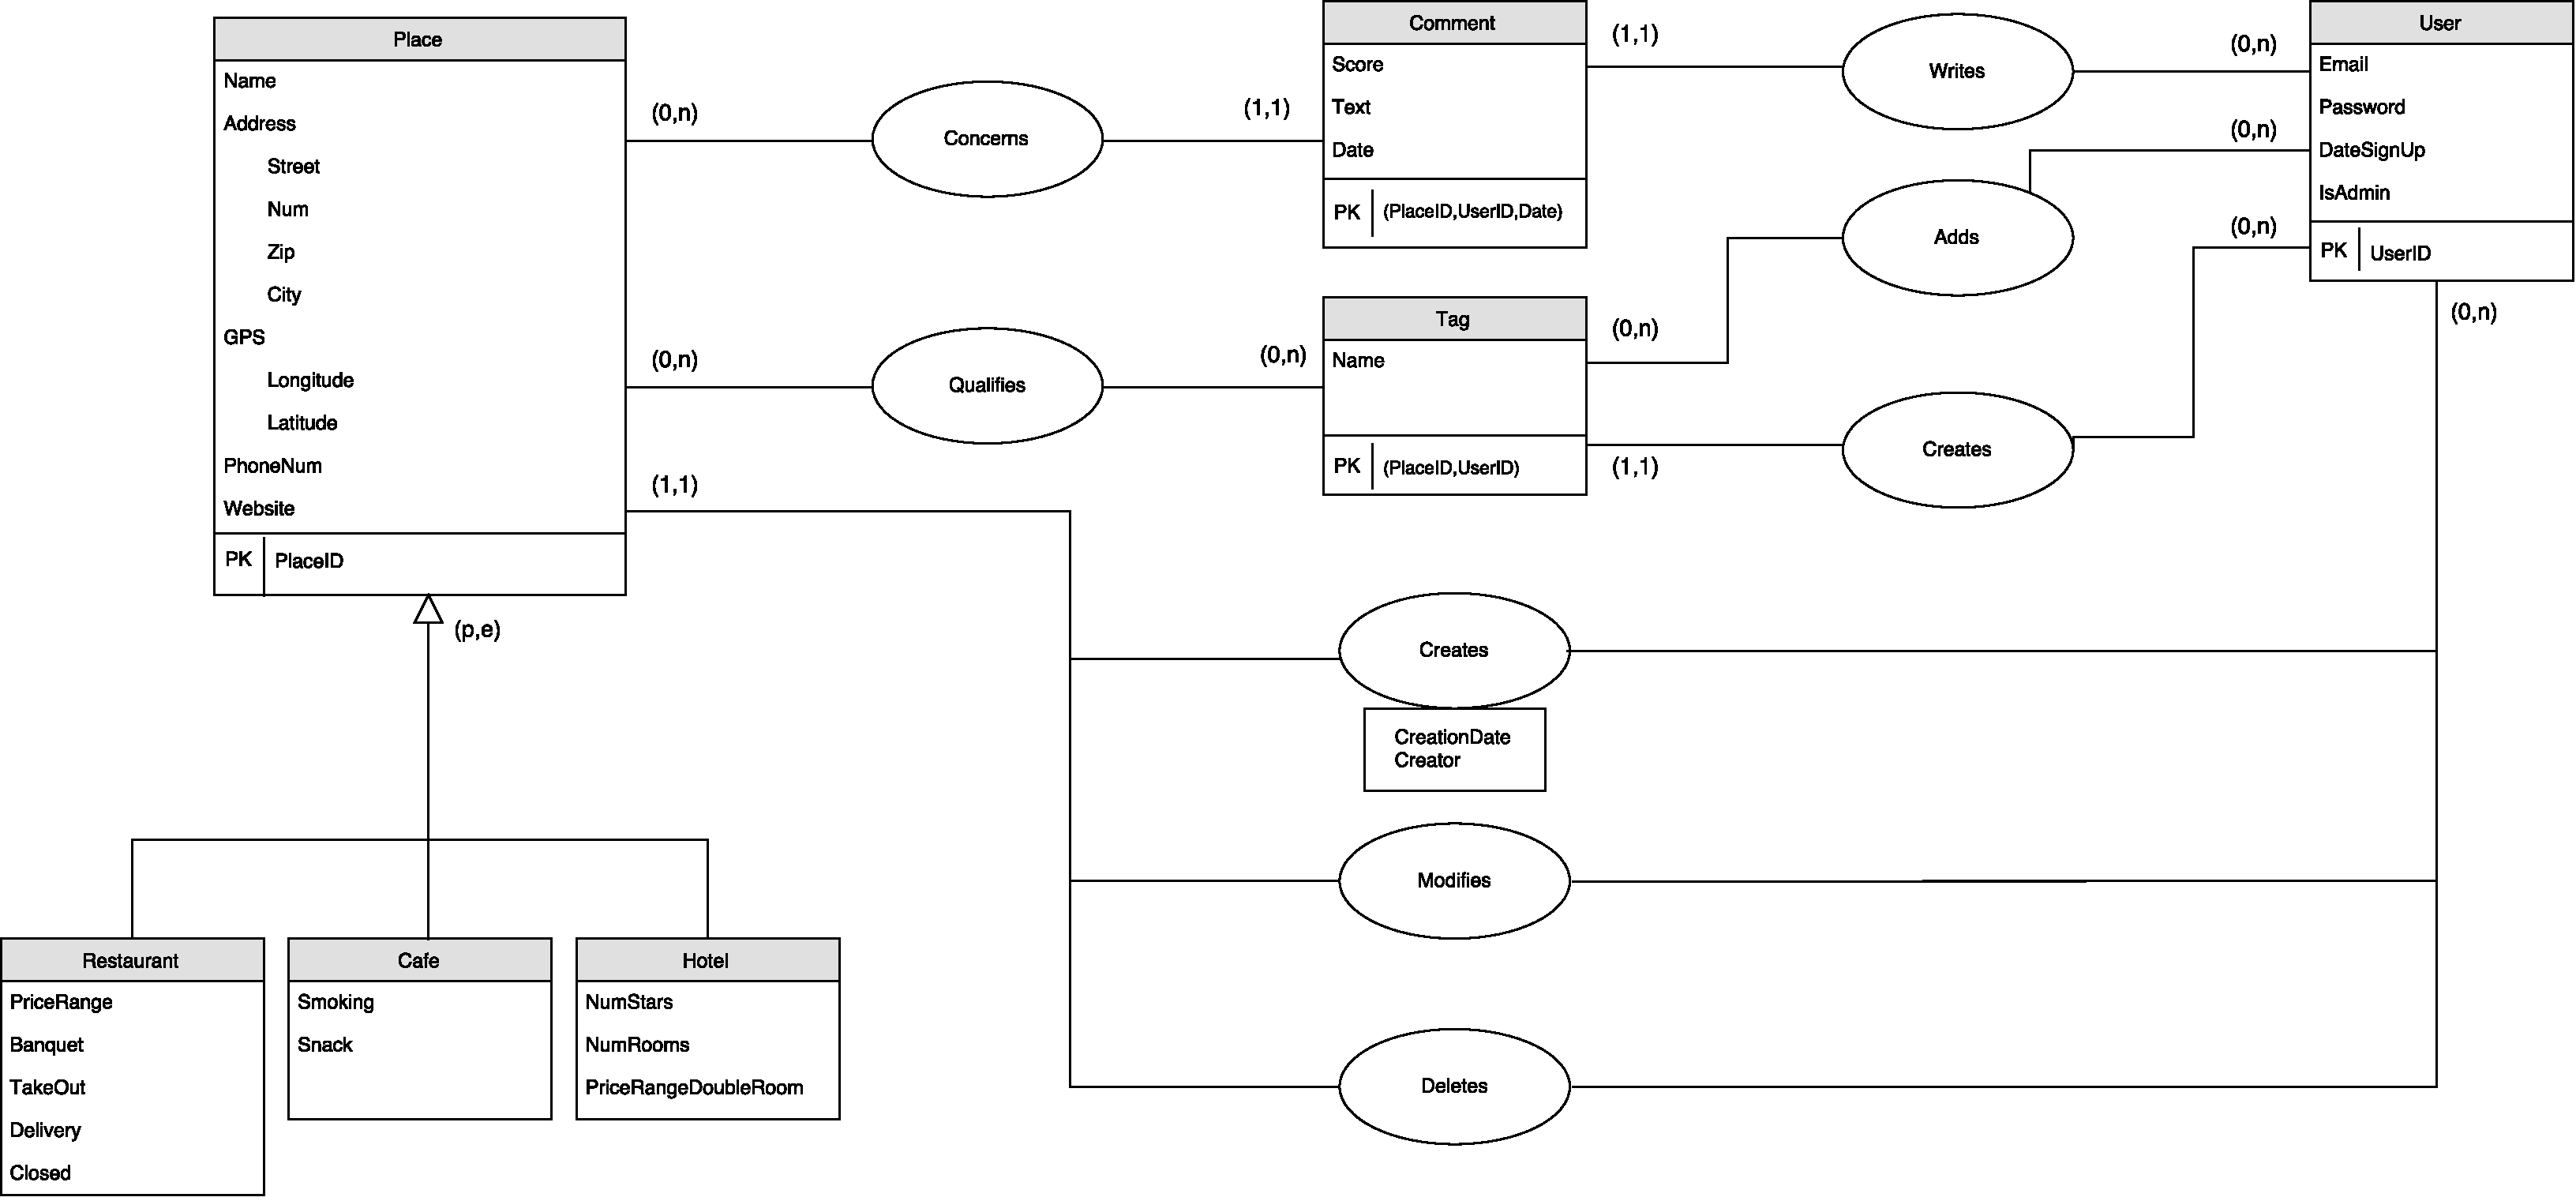
\includepdf[pages={-},angle=90,scale=0.97,pagecommand=\section{Diagramme entité-asssociation}\thispagestyle{empty}]{./../erdiagrams/ERDia.pdf}

\end{landscape}

\section{Traduction relationnelle}

\noindent User(\underline{ID}, Email, Password, DateSignUp, IsAdmin)

\hspace{-0,5cm}Place(\underline{ID}, Name, Address, GPS, PhoneNum, Website)

\hspace{-0,5cm}Restaurant(\underline{PID}, PriceRange, Banquet, TakeOut, Delivery, Closed)

PID reference Place.ID

\hspace{-0,5cm}Cafe(\underline{PID}, Smoking, Snack)

PID reference Place.ID

\hspace{-0,5cm}Hotel(\underline{PID}, NumStars, NumRooms, PriceRangeDoubleRoom)

PID reference Place.ID

\hspace{-0,5cm}Comment(\underline{PID}, \underline{UID}, \underline{Date}, Score, Text, Date)

PID reference Place.ID

UID reference User.ID

\hspace{-0,5cm}Tag(\underline{PID}, \underline{UID}, Name)

PID reference Place.ID

UID reference User.ID

\hspace{-0,5cm}Creates(\underline{PID}, \underline{UID}, CreationDate)

PID reference Place.ID

UID reference User.ID

\section{Contraintes d'intégrité}

\begin{itemize}
  \item Pour pouvoir créer, modifier ou supprimer un "Place", le "User" doit être un administrateur (\emph{IsAdmin} == True).
  \item La \emph{Date} d'un "Comment" doit être strictement supérieure à la \emph{CreationDate} d'un "Place".
  \item La \emph{Date} d'un "Comment" doit être strictement supérieure à la \emph{DateSignUp} du "User" qui le poste.
  \item Il ne peut exister deux "Comment" d'un même "User" pour un même "Place" à la même \emph{Date}.
  \item La \emph{Note} d'un "Comment" doit être comprise entre 0 et 5 inclus.
  \item Les \emph{Name} des "Tag" doivent être uniques.
  \item Un "User" ne peut apposer plus d'une fois un "Tag" sur une même "Place".
  \item Tous les \emph{Email} des "User" doivent être uniques.
\end{itemize}

\newpage

\section{Script SQL de création de la BDD}

\inputminted[bgcolor=black,firstline=1,lastline=50]{sql}{./../src/creation.sql}
\inputminted[bgcolor=black,firstline=51]{sql}{./../src/creation.sql}

\newpage

\section{Requêtes demandées}

\subsection{Requête 1}

\textbf{Tous les utilisateurs qui apprécient au moins 3 établissements que l’utilisateur "Brenda" apprécie.}

\subsubsection{SQL}

\begin{minted}{psql}
SELECT username FROM 
  (SELECT c.place_id, u.username FROM Comments  c 
   INNER JOIN Users u 
   ON c.user_id = u.user_id 
   WHERE c.stars > 3 AND username <> 'Brenda') a
INNER JOIN
  (SELECT c.place_id FROM Comments c 
   INNER JOIN Users u 
   ON c.user_id = u.user_id 
   WHERE c.stars > 3 AND u.username = 'Brenda') b
ON a.place_id = b.place_id
GROUP BY a.username HAVING count(username) >= 3;
\end{minted}

\subsubsection{Algèbre relationnelle}

$BrendaComments \leftarrow \sigma_{username\;\;=\;\;"Brenda"}\;(Users \bowtie_{user\_id=user\_id} Comments )$\\

$BrendaLikedPlaces \leftarrow \Pi_{place\_id} (\sigma_{stars>3}\;(BrendaComments))$ \\

$OtherComments \leftarrow \sigma_{username\;\; != \;\;"Brenda"} (Users \bowtie_{user\_id=user\_id} Comments )$\\

$SimilarTastesAsBrenda \leftarrow \sigma_{count(user\_id)>3}\; (OtherComments\bowtie_{place\_id=place\_id}BrendaLikedPlaces) $\\

$Solution \leftarrow \Pi_{username} (SimilarTastesAsBrenda) $

\subsubsection{Calcul relationnel tuple}

\newpage

\subsection{Requête 2}

\textbf{Tous les établissements qu’apprécie au moins un utilisateur qui apprécie tous les établissements que "Brenda" apprécie.}

\subsubsection{SQL}

\subsubsection{Algèbre relationnelle}

\subsubsection{Calcul relationnel tuple}

\newpage

\subsection{Requête 3}

\textbf{Tous les établissements pour lesquels il y a au plus un commentaire.}

\subsubsection{SQL}

\begin{minted}{psql}
SELECT a.name FROM Places a 
LEFT JOIN
  (SELECT DISTINCT place_id FROM Comments 
   GROUP BY place_id 
   HAVING count(place_id) > 1) b 
ON a.place_id = b.place_id 
WHERE b.place_id is null;
\end{minted}

\subsubsection{Algèbre relationnelle}


$ CommentedPlaces \leftarrow \Pi_{place\_id} (Comments) $ \\

$ LessCommentedPlaces \leftarrow \sigma_{count(place\_id) \leq 1} (Places \bowtie_{place\_id = place\_id} \; CommentedPlaces)$ \\

$ Solution \leftarrow \Pi_{name}(LessCommentedPlaces) $

\subsubsection{Calcul relationnel tuple}

\newpage

\subsection{Requête 4}

\textbf{La liste des administrateurs n’ayant pas commenté tous les établissements qu’ils ont crées.}

\subsubsection{SQL}

\subsubsection{Algèbre relationnelle}

\subsubsection{Calcul relationnel tuple}

\newpage

\subsection{Requête 5}

\textbf{La liste des établissements ayant au minimum trois commentaires, classée selon la moyenne des scores attribués.}

\subsubsection{SQL}

\subsection{Requête 6}

\textbf{La liste des labels étant appliqués à au moins 5 établissements, classée selon la moyenne des scores des établissements ayant ce label.}

\subsubsection{SQL}

\newpage

\section{Instructions d'installation de l'application}

\subsection{Dépendances}

Comme dit précédemment, le langage utilisé est Ruby. \footnote{Pour l'installer: \url{https://www.ruby-lang.org/en/downloads/} } Une installation de la version 2.0 au minimum est requise pour faire fonctionner l'application.

Il faut également installer PostgreSQL \footnote{Pour l'installer: \url{http://www.postgresql.org/download/} } , bien sur, qui est le gestionnaire de bases de données utilisé.

Pour gérer les dépendances et librairies Ruby utilisées dans le projet, il est nécessaire d'installer Bundle. \footnote{Pour l'installer: \url{http://bundler.io/} }

Une autre dépendance est Bower \footnote{\url{http://bower.io/}}, un gestionnaire de packages de frameworks et utilitaires web.

(LEAFLET.JS???)


\subsection{Installation}

Pour commencer l'installation, il faut aller dans le dossier contenant le code source de l'application et le fichier listant les dépendances.

\begin{minted}{bash}
cd Welp/src/welp
\end{minted}

Ensuite, deux commandes de bundle sont requises pour installer les dépendances.

\begin{minted}{bash}
bundle install --path vendor/bundle
(sudo) npm install bower -g
\end{minted}

À présent, il faut créer la base de données qui sera utilisée par l'application. Cette commande permets de créer une telle table, nommée ``welp''.

\begin{minted}{bash}
createuser --createdb --login -P welp
\end{minted}

Un menu apparaitra, il suffit de rentrer deux fois le mot de passe ``welp''.

Ensuite, on rentre dans le dossier ``db'' pour créer les tables de la base de données et la remplir avec les données initiales données avec l'énoncé du projet. Dans ce dossier ``db'' vous pouvez voir dans le sous-dossier ``migrate''. Le script SQL de création de la base de données, présenté plus haut, se trouve dans le fichier ``20160507141941\_create\_database.rb''. Il a été légèrement modifié pour que rails sache le parser.

\begin{minted}{bash}
cd db
ruby populate_seeds.rb
rake db:create db:migrate db:seed
\end{minted}

\section{Scénario de démonstration de l'application}

\section{Explications des choix et hypothèses}

\end{document}
